%%%%%% Kravspecifikation %%%%%%
%\newpage
\section{Funktionelle krav}
\label{sec:funkKrav}
De funktionelle krav beskrives via brugsscenarier, også kaldet use cases. Indledningsvis beskrives systemets aktører, og senere i afsnittet beskrives hvordan systemet fungerer ud fra interaktion mellem aktører og system.

\subsection{Aktør diagram}
%Følgende afsnit beskriver aktørerne i systemet.
Nedenstående figur viser hvilke aktører der interagerer med systemet.

\begin{figure}[H]
\centering
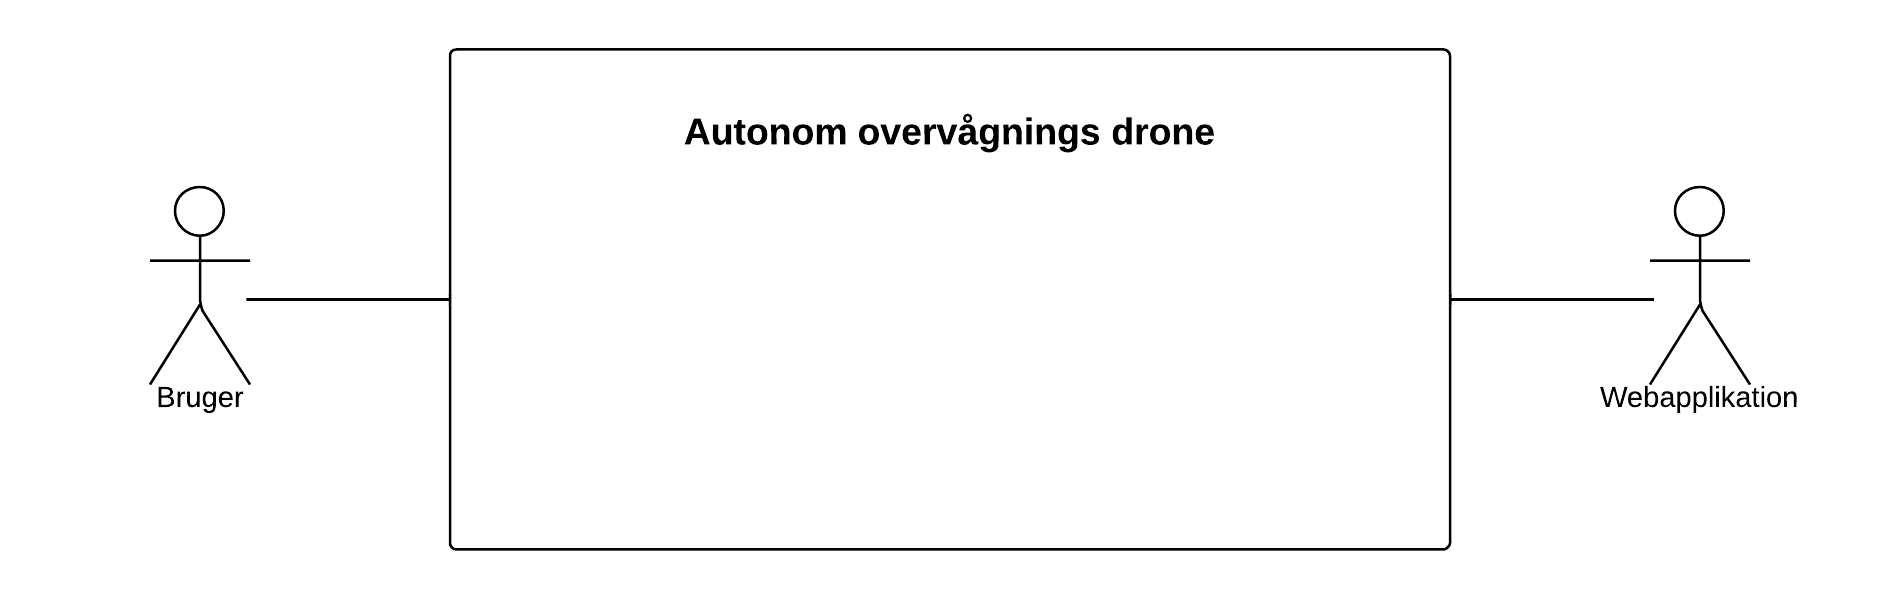
\includegraphics[width=1\textwidth]{Billeder/Aktor_diagram.png}
\caption{Aktør diagram}
\label{fig:ATD}
\end{figure}

\subsection{Aktørbeskrivelser}
Aktørbeskrivelsen skitserer systemets aktører samt hvilken rolle de spiller for systemet.


\begin{table}[H]
\begin{tabular}{|l|p{13.25cm}|} \hline

Navn					& Bruger. 	\\\hline
Type					& Primær.	\\\hline
Beskrivelse				& Bruger er den eneste person der interagerer med systemet.\\
						& Via webapplikation indstiller bruger flyveopsætning for nye flyvninger, \\ 
						& samt undersøge billeder og flyveruter fra tidligere flyvninger.\\\hline
						
\end{tabular}
\caption{Aktørbeskrivelse, Bruger}
\label{tab:AB1}
\end{table}


\begin{table}[H]
\begin{tabular}{|l|p{13.25cm}|}
\hline
Navn					& GPS satellitter. 	\\\hline
Type					& Sekundær.	\\\hline
Beskrivelse				& GPS satellitterne bruges når dronen lokaliserer sin position.\\\hline

\end{tabular}
\caption{Aktørbeskrivelse, GPS satellitter}
\label{tab:AB1}
\end{table}			

\newpage 

\subsection{Use case diagram}
\label{subsec:useCaseDiagram}
Figur \ref{fig:UCD} viser de identificerede use cases.
\vspace{-10pt}
%Usecase diagram indføres i følgende 5 linjer, derefter starter UC 1
\begin{figure}[H]
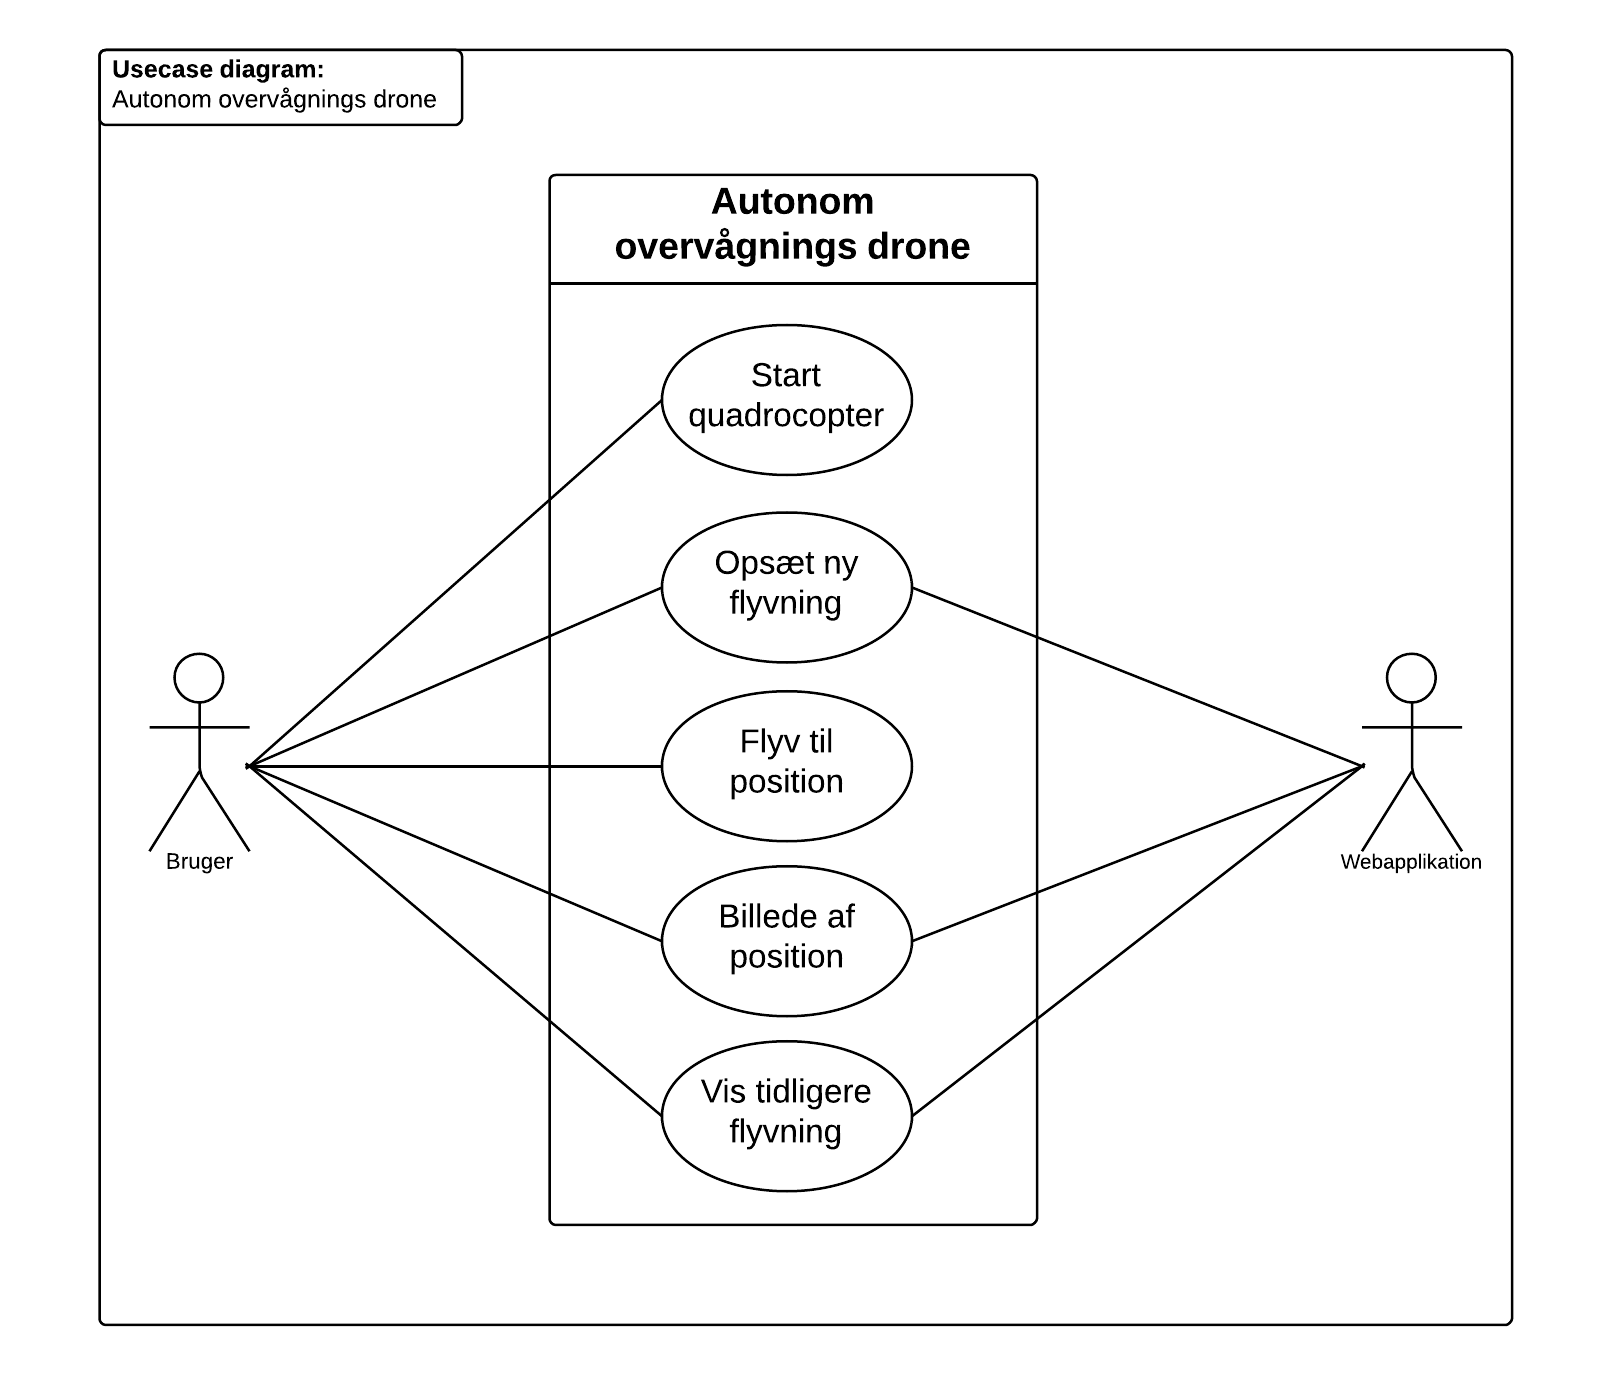
\includegraphics[width=1\textwidth]{Billeder/Use_case_diagram.png}
\vspace{-30pt}
\caption{Use case diagram}
\label{fig:UCD}
\end{figure}



\subsection{Udviklingsforløb}

For at tydeliggøre hvordan udviklingsforløbet  

\textbf{Iteration 1:}


\textbf{Iteration 2:}

\textbf{Iteration 3:}

\textbf{Iteration 4:}

\newpage
\subsection{Use case beskrivelse}
\label{subsec:useCaseBeskrivelse}
Fully dressed beskrivelse af de use cases der er vist i afsnit \ref{subsec:useCaseDiagram}. \newline 

\subsection*{UC1 - Start quadrocopter}

\begin{table}[H]
\begin{tabular}{|l|p{10cm}|}
\hline

Mål	 								& Quadrocopter er tændt og har forbindelse til webapplikation. \\\hline
Initiering 							& Bruger. \\\hline
Aktører og interesserede parter			& Bruger (primær) 
										\begin{itemize}
											\item Bruger tænder quadrocopter.
										\end{itemize} \\\hline
Startbetingelser						& Ingen. \\\hline
Slutbetingelser						& Quadrocopter er klar til at modtage flyveinstruktioner fra webapplikation. \\\hline
Hovedforløb				&
 
									\renewcommand{\labelenumi}{\arabic{enumi}.}
									\renewcommand{\labelenumii}{\Roman{enumii}:}

									\begin{enumerate}[topsep=0.0cm, leftmargin=0.5cm]
										\item Bruger tænder quadrocopter. 
										\item Quadrocopter initialiseres.
										\item Forbindelse fra quadrocopter til webapplikation oprettes.
											\begin{enumerate}[partopsep=4cm, topsep=0cm, leftmargin=1cm]
												\item Forbindelse kan ikke oprettes.
											\end{enumerate}
										
									\end{enumerate} \\\hline	

Undtagelser 							& 

									\renewcommand{\labelenumi}{\Roman{enumi}:}
									\renewcommand{\labelenumii}{\alph{enumii})}
									\begin{enumerate}[topsep=0.0cm,leftmargin=0.5cm]
										\item Forbindelse kan ikke oprettes.
											\begin{enumerate}[topsep=0cm, leftmargin=1cm]
												\item Systemet indikerer at der ikke er forbindelse mellem quadrocopter og webapplikation.
											\end{enumerate}
									\end{enumerate} \\\hline	

\end{tabular}
\caption{Use Case 1}
\label{tab:UC1}
\end{table}
\subsection*{UC2 - Ny flyveopsætning}

\begin{table}[H]
\begin{tabular}{|l|p{10cm}|}
\hline

Goal	 							& Ny flyveopsætning er oprettet og sendt til quadrocopter. \\\hline
Initiation 							& Bruger. \\\hline
No. of concurrent occurrence’s		& 1. \\\hline
Stakeholders	and Interests			& Bruger (primær) 
										\begin{itemize}
											\item Bruger ønsker at få adgang til webapplikation.
											\item Fra webapplikation indstiller bruger flyveopsætning.
										\end{itemize}
									  Webapplikation (sekundær)
										\begin{itemize}
											\item Sender flyveopsætning til quadropcopter.
										\end{itemize} \\\hline
Precondition							& Bruger er oprettet i systemet og UC\#1 er succesfuld gennemført  \\\hline
Postcondition						& Ny flyveopsætning er sendt til quadrocopter. \\\hline
Main success scenario				&
 
									\renewcommand{\labelenumi}{\arabic{enumi}.}
									\renewcommand{\labelenumii}{\Roman{enumii}:}

									\begin{enumerate}[topsep=0.0cm, leftmargin=0.5cm]
										\item Bruger logger på webapplikation.
										\begin{enumerate}[partopsep=4cm, topsep=0cm, leftmargin=1cm]
												\item Fejl i log-in.
										\end{enumerate}
										\item Efter succesfuld log-in vises webapplikations forside.
										\item Fra forsiden navigerer bruger til vindue hvorfra ny flyveopsætning indstilles.
									\end{enumerate} \\\hline	

Extensions							& 

									\renewcommand{\labelenumi}{\Roman{enumi}:}
									\renewcommand{\labelenumii}{\alph{enumii})}
									\begin{enumerate}[topsep=0.0cm,leftmargin=0.5cm]
										\item Fejl i log-in.
											\begin{enumerate}[topsep=0cm, leftmargin=1cm]
												\item Bruger bliver ført tilbage til log-in skærm.
											\end{enumerate}
									\end{enumerate} \\\hline	

\end{tabular}
\caption{Use Case 2}
\label{tab:UC2}
\end{table}
\subsection*{UC3 - Flyv til position}

\begin{table}[H]
\begin{tabular}{| p{3cm}| p{11.5cm}|}
\hline


Mål	 							& Drone flyver til ønsket position. \\\hline
Initiering 							& UC\#2 eller UC\#4. \\\hline
Aktører og \newline interesserede			& Bruger (primær) 

										\begin{itemize}
											\item Bruger ønsker at drone flyver som angivet i flyveopsætning.
										\end{itemize} \\  
										
										& GPS satellitter (sekundær) 

										\begin{itemize}
											\item Dronen opdaterer egen GPS position vha. GPS satellitterne.
										\end{itemize} \\ \hline
Startbetingelser							& UC\#1 og UC\#2 er succesfuld gennemført. \\\hline
Slutbetingelser						& Position er nået. \\\hline
Hovedforløb				&
 
									\renewcommand{\labelenumi}{\arabic{enumi}.}
									\renewcommand{\labelenumii}{\Roman{enumii}:}

									\begin{enumerate}[topsep=0.0cm, leftmargin=0.5cm]
										\item Nuværende position opdateres.
											\begin{enumerate}[partopsep=4cm, topsep=0cm, leftmargin=1cm]
												\item Ugyldig GPS koordinat.
											\end{enumerate}
										\item Flyvehøjde tilpasses.
											\begin{enumerate}[partopsep=4cm, topsep=0cm, leftmargin=1cm]
												\item Ugyldig flyvehøjde.
											\end{enumerate}
										\item Flyveorientering tilpasses.
										\item Drone flyver mod ønsket position.
									\end{enumerate} \\\hline	

Undtagelser							& 

									\renewcommand{\labelenumi}{\Roman{enumi}:}
									\renewcommand{\labelenumii}{\alph{enumii})}
									\begin{enumerate}[topsep=0.0cm,leftmargin=0.5cm]
										\item Ugyldig GPS koordinat.
											\begin{enumerate}[topsep=0cm, leftmargin=1cm]
												\item Drone går i fejlmode  \#1.
											\end{enumerate}
										\item Ugyldig flyvehøjde.
											\begin{enumerate}[topsep=0cm, leftmargin=1cm]
												\item Drone går i fejlmode \#2.
											\end{enumerate}
									\end{enumerate} \\\hline	

\end{tabular}
\caption{Use Case 3}
\label{tab:UC3}
\end{table}
\subsection*{UC4 - Billede af position}

\begin{table}[H]
\begin{tabular}{| p{3cm}| p{11.5cm}|}
\hline

Mål	 							& Quadrocopter tager et billede af nuværende position som sendes til webapplikation. Fra webapplikation kan bruger inspicere og acceptere billedet. \\\hline
Initiering 							& UC\#3. \\\hline
Aktører og interesserede			& Bruger (primær) 
										\begin{itemize}
											\item Kan inspicere og acceptere billede.
										\end{itemize} 
									  Webapplikation (sekundær)
										\begin{itemize}
											\item Modtager billede fra quadrocopter.
											\item Viser bruger billede der skal accepteres.
										\end{itemize} \\\hline
Startbetingelser							& UC\#1, UC\#2 og UC\#3 er succesfuld gennemført. \\\hline
Slutbetingelser						& 	\begin{itemize}
											\item Bruger kan tilgå billede via webapplikation.
											\item Quadrocopter flyver til næste GPS-position eller udgangsposition.
										\end{itemize} \\\hline
Hovedforløb				&
 
									\renewcommand{\labelenumi}{\arabic{enumi}.}
									\renewcommand{\labelenumii}{\Roman{enumii}:}

									\begin{enumerate}[topsep=0.0cm, leftmargin=0.5cm]
										\item Quadrocopter tager et billede af nuværende position.
										\item Billedet sendes til webapplikation.
										\item Bruger giver accept af billedet via webapplikation.
											\begin{enumerate}[partopsep=4cm, topsep=0cm, leftmargin=1cm]
												\item Bruger accepterer ikke billede.
												\item Bruger svarer ikke inden for tidsgrænsen.
											\end{enumerate}
										\item Quadrocopter sendes information om næste lokation.
									\end{enumerate} \\\hline	

Undtagelser							& 

									\renewcommand{\labelenumi}{\Roman{enumi}:}
									\renewcommand{\labelenumii}{\alph{enumii})}
									\begin{enumerate}[topsep=0.0cm,leftmargin=0.5cm]
										\item Bruger accepterer ikke billede.
											\begin{enumerate}[topsep=0cm, leftmargin=1cm]
												\item Quadrocopter instrueres til at ændre højde, orientering eller position. Derefter genstartes UC4.
											\end{enumerate}
										\item Bruger svarer ikke inden for tidsgrænsen.
											\begin{enumerate}[topsep=0cm, leftmargin=1cm]
												\item Quadrocopter får automatisk tildelt accept.
											\end{enumerate}
									\end{enumerate} \\\hline	

\end{tabular}
\caption{Use Case 4}
\label{tab:UC4}
\end{table}
\subsection*{UC5 - Billede af position}

\begin{table}[H]
\begin{tabular}{|l|p{10cm}|}
\hline

Goal	 								& Quadrocopter ankommer til position hvor den tager et billede som sendes til
webapplikation. Fra databasen kan bruger inspicerer og accepterer billedet. \\\hline
Initiation 							& UC\#4. \\\hline
No. of concurrent occurrence’s		& 1. \\\hline
Stakeholders	and Interests			& Bruger (primær) 
										\begin{itemize}
											\item Kan inspicerer og acceptere billede.
										\end{itemize} 
									  Webapplikation (sekundær)
										\begin{itemize}
											\item Modtager billede fra quadrocopter.
											\item Giver bruger billede der skal accepteres.
										\end{itemize} \\\hline
Precondition							& UC\#1, UC\#3 og UC\#4 er succesfuld gennemført. \\\hline
Postcondition						& 	\begin{itemize}
											\item Bruger kan tilgå flyverute og billede via webapplikation.
											\item Quadrocopter flyver til næste GPS-position eller udgangsposition.
										\end{itemize} \\\hline
Main success scenario				&
 
									\renewcommand{\labelenumi}{\arabic{enumi}.}
									\renewcommand{\labelenumii}{\Roman{enumii}:}

									\begin{enumerate}[topsep=0.0cm, leftmargin=0.5cm]
										\item Quadrocopter er ved ønsket GPS-koordinat og tager et billede.
										\item Billedet bearbejdes.
										\item Billedet sendes til webapplikation.
										\item Bruger er online på webapplikation og spørges om accept.
											\begin{enumerate}[partopsep=4cm, topsep=0cm, leftmargin=1cm]
												\item Bruger accepterer ikke billede.
												\item Bruger svarer ikke inden for tidsgrænsen.
											\end{enumerate}
										\item Quadrocopter flyver til næste GPS-position eller udgangsposition.
									\end{enumerate} \\\hline	

Extensions							& 

									\renewcommand{\labelenumi}{\Roman{enumi}:}
									\renewcommand{\labelenumii}{\alph{enumii})}
									\begin{enumerate}[topsep=0.0cm,leftmargin=0.5cm]
										\item Bruger accepterer ikke billede.
											\begin{enumerate}[topsep=0cm, leftmargin=1cm]
												\item Quadrocopter instrueres til at ændre højde, orientering eller position Trin 1-4 i main succes scenario gentages indtil bruger accepterer billede.
											\end{enumerate}
										\item Bruger svarer ikke inden for tidsgrænsen.
											\begin{enumerate}[topsep=0cm, leftmargin=1cm]
												\item Quadrocopter får automatisk tildelt accept og sendes instruktioner om atflyve næste GPS-position eller til udgangsposition.
											\end{enumerate}
									\end{enumerate} \\\hline	

\end{tabular}
\caption{Use Case 05}
\label{tab:UC05}
\end{table}
\subsection*{UC6 - Anti kollision}

\begin{table}[H]
\begin{tabular}{| p{3cm}| p{11.5cm}|}
\hline

Mål	 								& Drone kan undvige forhindringer. \\\hline
Initiering 							& Ingen - altid aktiv. \\\hline
Aktører og \newline stakeholders		& Bruger (stakeholder) 
										\begin{itemize}
											\item Ønsker flyvning uden kollision.
										\end{itemize} \\\hline
Startbetingelser							& UC\#3 er igangværende. \\\hline
Slutbetingelser						& Drone undviger en kollision. \\\hline

Hovedforløb				&
 
									\renewcommand{\labelenumi}{\arabic{enumi}.}
									\renewcommand{\labelenumii}{\Roman{enumii}:}

									\begin{enumerate}[topsep=0.0cm, leftmargin=0.5cm]

										\item Anti kollision detekterer en forhindring.
										\item Undvigningsmanøvre udføres.
											\begin{enumerate}[a:,topsep=0cm, leftmargin=1cm]
												\item Forhindring kan ikke undviges.
											\end{enumerate}
									\end{enumerate} \\\hline	

Undtagelser							& 

									\renewcommand{\labelenumi}{\Roman{enumi}:}
									\renewcommand{\labelenumii}{\alph{enumii})}
									\begin{enumerate}[a:,topsep=0.0cm,leftmargin=0.5cm]
										\item Forhindring kan ikke undviges.
											\begin{itemize}[topsep=0cm, leftmargin=1cm]
												\item Drone går i fejlmode \#3.
											\end{itemize}
									\end{enumerate} \\\hline	

\end{tabular}
\caption{Use Case 6}
\label{tab:UC6}
\end{table}

\newpage
\section{Ikke-funktionelle krav}
\label{sec:ikkeFunkKrav}
De ikke-funktionelle krav indeholder specifikke krav som timings, afstande og lydniveauer.
Ikke-funktionelle inddeles i følgende 3 grupper: Generelle krav, krav til webapplikation og krav til quadrocopter.\newline


\begin{enumerate}
\item \textbf{Generelle krav}
	\begin{enumerate}[label*=\arabic*.]
	\item Kommunikation mellem quadrocopter og webapplikation skal foregå trådløst.
	\item Trådløs kommunikation benytter 3G protokol eller ældre. 
	\item Højdemåler skal måle højde $\pm$ 10 cm.\\
	\end{enumerate}

\item \textbf{Krav til webapplikation}
	\begin{enumerate}[label*=\arabic*.]
	\item Webapplikation skal kunne tilgås via både computere og telefoner.
	\item Indholder database med billeder og flyveruter fra tidligere.
	\item Indholder database med brugere.\\
	\end{enumerate}	
	

\item \textbf{Krav til quadrocopter}
	\begin{enumerate}[label*=\arabic*.]
	\item Skal forsynes fra batteri.
	\item Batterilevetiden skal minimum være 15 minutter.
	\item Flyvehastigheden skal minimum være 2$\frac{m}{s}$.
	\item Flyvehøjde kan reguleres mellem 1 og 2,5 meter.
	\item Højde der tages billeder fra, kan reguleres mellem 1 og 2,5 meter.\\
	
	\end{enumerate}
	
\item \textbf{Krav til opsamling af data}
	\begin{enumerate} [label*=\arabic*.]
	\item Gyldig højdemåling ligger i intervallet 0,5 til 4,5 meter. 
	\item GPS skal angive koordinat indenfor $\pm$ 2,5 meter.
	\end{enumerate}
\end{enumerate}